% !TeX spellcheck = en_US
\documentclass[french]{yLectureNote}

\title{Atomistique}
\subtitle{La matière à l'échelle atomique}
\author{Paulhenry Saux}
\date{\today}
\yLanguage{Français}

\professor{J.Cuny}%sebastien.deveuhels.irap.omp.eu

\usepackage{graphicx}%----pour mettre des images
\usepackage[utf8]{inputenc}%---encodage
\usepackage{geometry}%---pour modifier les tailles et mettre a4paper
%\usepackage{awesomebox}%---pour les boites d'exercices, de pbq et de croquis ---d\'esactiv\'e pour les TP de PC
\usepackage{tikz}%---pour deiffner + d\'ependance de chemfig
\usepackage{tkz-tab}
\usepackage{chemfig}%---pour deiffner formules chimiques
\usepackage{chemformula}%---pour les formules chimiques en \'equation : \ch{...}
\usepackage{tabularx}%---pour dimensionner automatiquement les tableaux avec variable X
\usepackage{awesomebox}%---Pour les boites info, danger et autres
\usepackage{menukeys}%---Pour deiffner les touches de Calculatrice
\usepackage{fancyhdr}%---pour les en-t\^ete personnalis\'ees
\usepackage{blindtext}%---pour les liens
\usepackage{hyperref}%---pour les liens (\`a mettre en dernier)
\usepackage{caption}%---pour la francisation de la l\'egende table vers Tableau
\usepackage{pifont}
\usepackage{array}%---pour les tableaux
\usepackage{lipsum}
\usepackage{yFlatTable}
\usepackage{multicol}
\newcommand{\Lim}[1]{\lim\limits_{\substack{#1}}\:}
\renewcommand{\vec}{\overrightarrow}
\begin{document}
\setcounter{chapter}{1}

	\chapter{Spectre d'émission de l'atome d'hydrogène}

\section{Structure électronique de l'atome d'hydrogène}
\subsection{Caractéristiques}
Hydrogène : 1 proton

Deutérium : 1 proton + 1 neutron

Tritium : 1 proton + 2 neutrons

C'est l'élément le plus abondant de l'univers (92\%).
\subsection{Spectre d'émission}
Dispersion de la lumière émise par un prise : on obtient des raies de couleurs : c'est un spectre discret de couleur, non continue. On observe ainsi que l'énergie de l'électron est discontinue. Un électron ne peut pas avoir toutes les énergies mais certaines bien déterminées. Cela s'oppose au modèle de Rhuterford.
\subsubsection{La lumière}
La lumière est une onde, décrite par leur longueur d'onde. L'infrarouge à moins d'énergie que l'ultraviolet.
\begin{theorem}[Fréquence]
\[\nu_{(Hz = s^{-1})} = \frac{c_{(m\cdot s^{-1})}}{\lambda_{(m)}}\]
\end{theorem}

\begin{theorem}[Relation de Planck]
\[E = \frac{hc}{\nu} = h_{(J\cdot s)}\nu\]
\end{theorem}
\section{Modèle de Bhor}
Il existe des orbites stables pour lesquelles l'électron ne rayonne aucune énergie

Ces orbites correspondent à des niveaux d'énergie.

Elles sont caractérisées par leur moment angulaire en orbite, qui s'écrit L = n h barré

Utile pour l'énergie et spectre de H sont assez bons.

Mais mauvaise distance électron-noyau pour niveaux excités

Mauvaise description des autres atomes.

\subsection{États}
État fondamental = Étal de plus basse énergie (n=1)
États excités : tous les états avec une énergie supérieure à l'état fondamental. Il y a en a une infinité.

\checkInfo{Lampe à Hydrogène}{Les électrons sont excités par l'énergie donc ils passent dans un état supérieur. cependant l'état n'est pas stable. Donc il passe à un niveau d'énergie inférieur en émettant un photon}

Pour passer à un niveau d'énergie supérieur, il doit absorber un photon fournissant exactement l'énergie nécessaire.\marginCritical{Ce n'est pas l'intensité qui compte mais la longueur d'onde.}  Réciproquement, pour redescendre, il émet un photon d'un certain niveau d'énergie.
\subsubsection{Énergie d'un État}
\begin{theorem}[Uniquement pour l'hydrogène]
\[E_n = -\frac{hcR_H}{n^2}\] avec n le nombre quantique principal, $1 \leq$ et $R_H$ la constante de Rydberg
\end{theorem}
Ici, $hcR_H = 2.17\cdot10^{-18} = 13.598eV$. Donc \[E_n = -\frac{13.6}{n^2}eV\]
\begin{theorem}[Uniquement pour les hydrogénoides]
\[E_n = -\frac{hcR_HZ^2}{n^2} = -\frac{13.6\times Z^2}{n^2}eV\]
\end{theorem}
\subsubsection{Lien avec les raies d'émission}

\begin{flalign*}
E_{ph} &=\frac{hc}{\lambda}\\
&= E_n' - E_n\\
&=hcR_H(-\frac{1}{n'^2} + \frac{1}{n^2})\\
&\Rightarrow \frac{1}{\lambda} = R_H(-\frac{1}{n'^2} + \frac{1}{n^2})\\
&\Rightarrow \lambda = \frac{1}{R_H(-\frac{1}{n'^2} + \frac{1}{n^2})}
\end{flalign*}
On a $n'>n$ pour l'émission.\marginCritical{
$n'$ correspond toujours au niveau le plus et $n$ au niveau le plus. Ainsi, dans le cas :
\begin{itemize}
 \item d'une émission de photon : $n$ est le niveau de départ et $n'$ celui d'arrivée
  \item d'une absorption de photon : $n$ est le niveau d'arrivée et $n'$ celui de départ
\end{itemize}}
Dem pour trouver $n$ et $n'$.
\tipsInfo{Séries d'émissions principales}{
	\begin{tabular}{_l^l^l}
		\tableHeaderStyle%
		Série de & Excitation vers n= & Domaine\\
		Balmer & 2 & Visible\\
		Lyman & 1 & Ultraviolet\\
		Paschen, Brackett, Pfund & $\geq$3 & Infrarouge\\
	\end{tabular}}
\subsubsection{Lien avec l'énergie}
La transition d’un niveau d’énergie plus élevé vers un état fondamental (telle que de la couche 3 à la couche 1) produit un photon d’énergie plus élevée que la transition d’un état de départ inférieur (de 2 à 1).\marginCritical{Cela signifie que la longueur d'onde sera plus petite car $\lambda = \frac{hc}{E}$}

À l'inverse la transition de l' état fondamental vers un niveau d'énergie élevé (telle que de la couche 1 à la couche 3) demande un photon d’énergie plus élevée que la transition vers un état d'arrivée inférieur (de 1 à 2).\marginCritical{Cela signifie que la longueur d'onde sera plus grande car $\lambda = \frac{hc}{E}$}
\subsubsection{Ionisation}
\begin{theorem}[Définition de l'énergie de ionisation]
La valeur minimale de
l’énergie qu’il faut fournir à l’atome d’hydrogène pris dans son état fondamental pour lui
arracher son électron. $E_i = -E_1$.
\end{theorem}
\subsection{Méthodes}
\subsubsection{Déterminer un niveau de transition}
On conna\^it la longueur d'onde associée à la transition et le niveau le plus bas.
\begin{flalign*}
\frac{1}{\lambda} &= R_H(-\frac{1}{n'^2} + \frac{1}{n^2})\\
\frac{1}{\lambda R_H} &= -\frac{1}{n'^2} + \frac{1}{n^2}\\
\frac{1}{\lambda R_H} -\frac{1}{n^2}&= -\frac{1}{n'^2}\\
\frac{-1}{\lambda R_H} +\frac{1}{n^2}&= \frac{1}{n'^2}\\
\frac{-n^2}{\lambda R_H n^2} +\frac{\lambda R_H}{n^2\lambda R_H}&= \frac{1}{n'^2}\\
\frac{\lambda R_H -n^2}{\lambda R_H n^2}&= \frac{1}{n'^2}\\
\sqrt{\frac{\lambda R_H n^2}{\lambda R_H -n^2}}&= n'\\
\end{flalign*}

On conna\^it la longueur d'onde associée à la transition et le niveau le plus haut.

\begin{flalign*}
\frac{1}{\lambda} &= R_H(-\frac{1}{n'^2} + \frac{1}{n^2})\\
\frac{1}{\lambda R_H} &= -\frac{1}{n'^2} + \frac{1}{n^2}\\
\frac{1}{\lambda R_H} +\frac{1}{n'^2}&= \frac{1}{n^2}\\
\frac{\lambda R_H +n'^2}{\lambda R_H n'^2}&= \frac{1}{n^2}\\
\sqrt{\frac{\lambda R_H n'^2}{\lambda R_H +n'^2}}&= n\\
\end{flalign*}
\subsubsection{Déterminer un niveau d'énergie à partir d'une énergie reçue}
On peut transformer l'énergie en longueur d'onde avec $\displaystyle E = h\frac{c}{\lambda}$, puis utiliser les méthodes précédentes.

On peut utiliser la formule de base :
\begin{flalign*}
E_n &= -\frac{hcR_H}{n^2}\\
n &= \sqrt{\frac{-hcR_H}{E_n}}
\end{flalign*}
\subsubsection{Déterminer les transition possibles une fois que l'atome est soumis à une certaine énergie}
On détermine le niveau d'énergie sur lequel il se trouve avec la méthode précédente.

Ce sont toutes les transitions amenant à un niveau inférieur. Il y en a $\sum^n_{k=1} (n-1)$
\subsubsection{Déterminer l'énergie d'ionisation d'un hydrogénoide}
Elle dépend du niveau dans lequel se trouve l'électron. Si ce n'est pas précisé, on le suppose dans l'état fondamental et $n=1$.

$\displaystyle E_{\infty} = - E_n =  \frac{hcR_H}{n^2}Z^2$ avec $Z$ le nombre de protons et $n$ l'énergie du niveau dans lequel se trouve l'électron.

\subsubsection{Déterminer une transition électronique à partir d'une longueur d'onde chez un hydrogénoide}
On suppose qu'il est dans l'état fondamental à l'origine.

On a l'égalité : \[E_n = -\frac{hcR_H}{n^2}Z^2 = E_1 + E_{ph} = - \frac{hcR_H}{1}Z^2 + E_{ph} \]

On en tire la valeur de n : \[ n = \frac{-hcR_HZ^2}{-hcR_H + E_{ph}} \] avec $E_{ph}$ l'énergie d'un photon que l'on retrouve avec $E = h\frac{c}{\lambda}$.\marginCritical{Cette expression met en jeu l'énergie d'un photon que l'on obtient en Joules avec la relation $E = h\frac{c}{\lambda}$. Il faut donc le convertir en eV pour effectuer le calcul.}
\section{Équation de Schrödinger}
\subsection{Intro}
Dés qu'on a plusieurs électrons, le modèle de Bhor ne fonctionne plus. Dans le modèle de la mécanique quantique, les électrons sont décrits par des fonctions d'onde. Dans le cas des électrons de l'atome, les fonctions d'ondes sont appelées orbitales atomiques. Les OA sont les solutions des équations de shrodinger indépendantes du temps.
\subsection{Modèle de Schrödinger}
On ne peut pas connaître la position d'un électron : probabilité de présence

L'électron occupe une orbitale atomique définie par son énergie et sa forme.
\subsubsection{Nombres quantiques}
Pour chaque couche n, il existe $n^2$ Orbitales atomiques. Chaque OA est caractérisée par 3 nombres quantiques : n, l et ml. Ce sont des entiers.


Une couche est l'ensemble des m\^emes OA avec le m\^eme n. Il y a $n^2$ orbitales atomiques pour n = 2.

	\begin{tabular}{_l^l^l^l}
		\tableHeaderStyle%
		Nombre & Utilité & valeurs & Nombre de valeurs\\
		n & énergie/taille de l'orbitale & 1.2.3& n\\
		l & forme de l'orbitale & 0,1,2,...,(n-1)&n\\
		ml & orientation de l'orbitale & l,l-1,...,1,0,-1,...-(l-1),-l&(2l+1)\\
	\end{tabular}
\subsubsection{Représentations graphiques}
Il y a 3 variables donc 4 dimensions. Il faut donc des outils pour les représenter en 3 dimension.
\warningInfo{Modes de représentation : Isosurface et nuage de probabilité}{On utilise des isosurfaces (On relie tous les points de l'espace qui ont la m\^eme valeur, choisie arbitrairement), où un nuage de probabilité de présence de l'électron (plus il y a de points présents dans une zone, plus l'elctron à de chances de s'y trouver).}

La fonction peut \^etre positive ou négative. Les couleurs représentent le signe de la fonction.\marginCritical{L'électron est toujours négatif. Le spin n'est pas non plus influencé par le signe de la fonction. La forme de la fonction ne représente pas non plus un mur dans lequel l'électron se trouve. La fonction OA a des valeurs partout.}

On étudie les probabilités que l'électron soit dans un volume donné
\subsubsection{Énergie}
Pour les hydrogénoides :
\begin{itemize}
 \item On ne remet pas en couse le modèle de Bhor, qui s'avère juste
 \item Chaque niveau a plusieurs OA, avec le m\^eme $n$ et donc la m\^eme énergie $E_n$ car l'énergie ne dépend que de $n$ pour les hydrogénoides.
\end{itemize}

En revanche, avec plusieurs électrons, il y a une levée de dégénérescence : Les sous-couches d'une m\^eme couche n'ont plus la m\^eme énergie.

\subsubsection{Nomenclature des sous-couches}
XY avec X = n et Y : Voir tableau pour la corresponde l$\rightarrow$lettre.

	\begin{tabular}{_c^c}
		\tableHeaderStyle%
		valeur de l & lettre correspondante \\
		0 & s\\
		1 & p\\
		2 & d\\
		3 & f\\
		4 & g\\
		5 & h\\
	\end{tabular}

	Une sous-couche est un ensemble d'OA
	\subsection{Le spin}
	\subsubsection{Expérience de Stern et Gerlach : }
	Une source d'atome d'argent que l'on fait passer dans un champ magnétique inhomogène (qui à des valeurs différentes dans l'espace). On récupère 2 taches.
\subsubsection{Définition}
	Il y a un moment magnétique dans l'électron et donc un moment cinétique, intrinsèque à l'atome. Il existe un 4e nombre quantique qui quantifie le moment cinétique intrinsèque, qui existe pour toute particules. quantiques\marginCritical{Il ne faut pas confondre le nombre quantique de spin, le spin (=moment cinétique intrisèque) et le nombre magnétique de spin.} :
	\begin{itemize}
	 \item le nombre quantique de spin, noté s pour l'électron. Il vaut $\frac{1}{2}$. (Les fermions ont un nombre demi-entier)
	 \item le nombre quantique magnétique de spin, $m_s$, qui ne peut prendre que $2s+1$ valeurs. Il peut prendre 2 valeurs $\pm\frac{1}{2}$
	\end{itemize}
	\subsection{Règle de Pauli}
Selon Pauli, Dans la fonction d'onde, si j'inverse 2 électrons, cela génère un -.\marginInfo{Il l'a dit selon ces termes : ``La fonction d'onde d'un système fermionique est antisymétrique par permutation''}
\criticalInfo{Conséquence}{Dans l'atome, 2 électrons ne peuvent pas avoir leur 4 nombre quantique identique. Une OA ne peut donc décrire que 2 électrons}

\section{Présentation des fonctions}
\subsection{Orbitale atomique}
$\hat{H}\Psi(r,\theta,\varphi) = E\Psi(r,\theta,\varphi)$. Les orbitales atomiques sont les solutions de cette équation.
On a : \[\Psi = R_{n,l}(r)Y_{l,ml}(\theta,\varphi)\]

La partie radiale est une exponentielle décroissante mais la partie angulaire est une exponentielle complexe.
\subsection{Coordonnées sphériques}
Voir Outils Maths mais Propriétés importantes :
\begin{itemize}
 \item $\mathrm{d}v = r^2\mathrm{d}r \sin\theta \mathrm{d}\theta \mathrm{d} \varphi$
 \item $\theta : 0 \rightarrow \pi$
 \item $\varphi : 0 \rightarrow 2\pi$
\end{itemize}



\subsection{Sens physique de la fonction d'onde}
	\begin{tabular}{_l^l^l}
		\tableHeaderStyle%
		Expression & Sens & Unité\\
		$\Psi(r,\theta,\varphi)$ & Aucun & m$^{-3/2}$ \\
		$|\Psi(r,\theta,\varphi)|^2$ &  densité de probabilité de présence de l'électron au point $r,\theta,\varphi$ & m$^{-3}$\\
		$|\Psi(r,\theta,\varphi)|^2 d\tau$ & Probabilité infinitésimale & m$^{-3}$\\
		$\int\int\int|\Psi(r,\theta,\varphi)|^2 d\tau$ & Probabilité pour un certain volume & m$^{-3}$\\
	\end{tabular}
\subsection{Intégration}
On intègre normalement :
$\int_r\int_{\theta}\int_{\varphi}|\Psi(r,\theta,\varphi)|^2 d\tau$

On intègre maintenant sur tout l'espace :
$\int_0^{+\infty}\int_0^{\pi}\int_0^{2\pi}|\Psi(r,\theta,\varphi)|^2 d\tau = 1$
\warningInfo{}{Toutes les fonctions d'onde sont normalisées car l'intégrale sur tout l'espace fait 1.
}
On remplace maintennt par l'expression de la fonction : $\int_0^{+\infty}\int_0^{\pi}\int_0^{2\pi}|R_{n,l}(n)Y_{m,ml}(\theta,\varphi)|^2 d\tau = 1$

$\int_0^{+\infty}\int_0^{\pi}\int_0^{2\pi}|R_{n,l}(n)|^2|Y_{l,ml}(\theta,\varphi)|^2 d\tau = 1$

On enlève le module sur $R$ car la fonction est toujours réelle :
$\int_0^{+\infty}\int_0^{\pi}\int_0^{2\pi}R_{n,l}(n)^2|Y_{l,ml}(\theta,\varphi)|^2 d\tau = 1$

On remplace la quantité infinitésimale :

$\int_0^{+\infty}\int_0^{\pi}\int_0^{2\pi}R_{n,l}(n)^2|Y_{l,ml}(\theta,\varphi)|^2 r^2\mathrm{d}r \sin\theta \mathrm{d}\theta \mathrm{d} \varphi  = 1$

On sépare l'intégrale en fonction des variables :

\[\int_0^{+\infty}R_{n,l}(n)^2 r^2\mathrm{d}r \int_0^{\pi}\int_0^{2\pi}|Y_{l,ml}(\theta,\varphi)|^2  \sin\theta \mathrm{d}\theta \mathrm{d} \varphi  = 1\]

\checkInfo{Traduction des intégrales}{La première est la condition de normalisation radiale et la deuxième est la condition de normalisation angulaire}
\subsection{Raisonnement inverse}
\begin{enumerate}
 \item $\int_0^{+\infty}R_{n,l}(n)^2 r^2\mathrm{d}r$ est une probabilité radiale, c'est à dire la probabilité que l'atome se trouve à une certaine distance.
 \item $R_{n,l}(n)^2 r^2\mathrm{d}r$ est une probabilité infinitésimale.
 \item $R_{n,l}(n)^2 r^2$ est une densité de probabilité radiale.
\end{enumerate}
\section{Étude des fonctions}
\subsection{Fonction radiale}
$R_{n,l}(n)^2 r^2$ est toujours nulle à l'origine. Les valeurs nulles en dehors de celle à l'origine de la fonction sont appelés noeuds radiaux. Le nombre de noeuds est donné par : $R_{n,l}(r) = n-l-1$
\warningInfo{Noeud radial}{C'est une distance au noyau pour lequel la densité de probabilité de présence de l'électron est nulle.}

Pour décrire où un électron peut se trouver, il faut utiliser $|R_{n,l}(n)|^2 r^2$ dont l'intégrale est normalisée.
\warningInfo{Représentations}{Un minimum de $R(r)^2r^2$ indique qu'il y a un noeud radial, donc une valeur nulle sur $R(r)$ !}
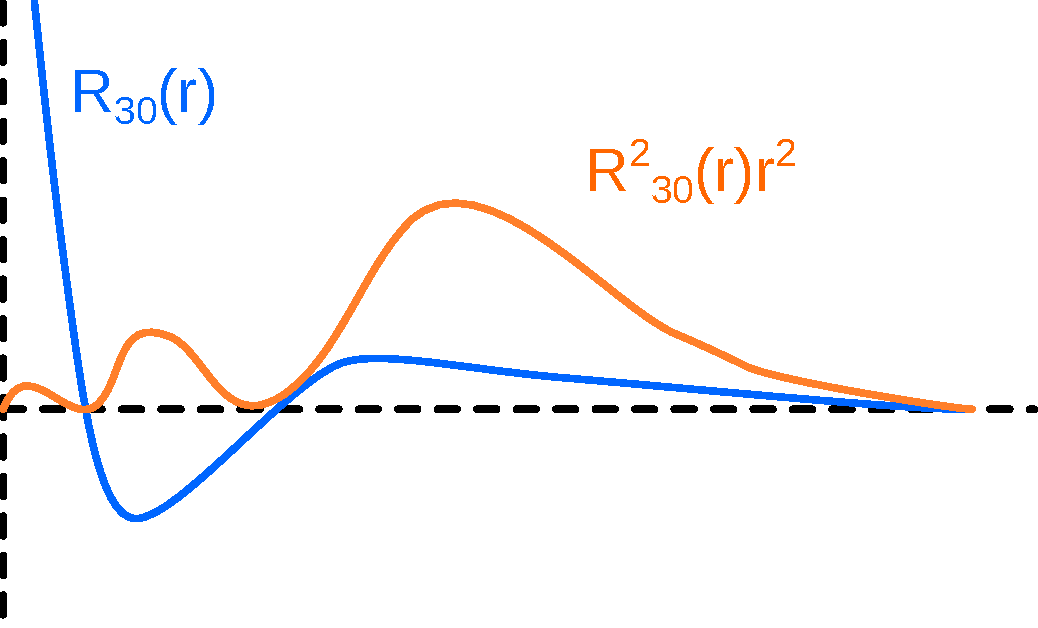
\includegraphics[scale=0.5]{OA-rad}
\subsection{Partie angulaire}
Elles sont aussi normalisées

On fait des combinaisons linéaires de$\pm m_l$ pour trouver des fonctions réelles que l'on peut représenter
\warningInfo{Zéros de la partie radiale}{Comme la fonction angulaire a 2 variable, les zéros sont des plans, appelé surfaces nodales.}

%La partie angulaire à $l-|m|$ noeuds}


On peut déterminer la sous-couche de la représentation en déterminant le nombre de surfaces nodales présentes sur une symétrie. \marginCritical{Par exemple, sur le membre de droite des représentations des OA de type $p$, il y a une symétrie pour n=2, 2 pour n=3 et 3 pour n=4. De cette manière, on peut déterminer $n$. Pour le type $p$, il y a une symétrie pour n=3 et 2 pour n=3. }


\subsection{Assemblage des 2}
Quand on change la partie radiale, l'OA change de taille et on rajoute des noeuds radiaux.
\criticalInfo{}{Toutes les orbitales atomiques sont définies au signe près.}
\subsection{Sur les noeuds}
Il faut différentier les noeds sphériques correspondant aux zéros de la fonction radiale et les noeuds plans (donnés par la fonction angulaire).

Le nombre de noeud sphérique est donné par $n-l-1$ et les noeuds angulaires sont donnés par $l$.

On a donc :

\begin{tabular}{_c^c^c}
		\tableHeaderStyle%
		Orbitales & Noeuds plans = angulaire & Noeuds sphériques = radiaux\\
		s & 0 & n-1\\
		p & 1 & n-2\\
		d & 2 & n-3\\
	\end{tabular}

	Ici, le noeud rouge représente le noeud radial et le jaune le noeud angulaire :

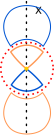
\includegraphics[scale=0.4]{noeuds}

\subsection{Multiplication des 2 fonctions}
Lorsque l'on multiplie la partie angulaire avec la partie radiale, 2 choses se produisent :
\begin{itemize}
\item L'OA s'agrandit
\item Elle se sépare selon les points nodaux de R : un nouveau noeud sphérique apparait
\end{itemize}

Pour passer de l'OA $2p$ à l'OA $3p$, on regarde la représentation de $R_3,1(r)$ et on observe un noeud radial à une distance $a$.

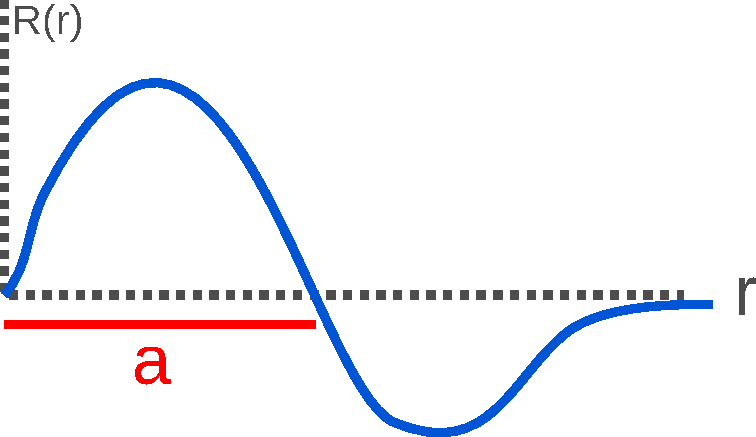
\includegraphics[scale=0.5]{3p-r}

Ainsi, on aura une nouvelle surface nodale sur la représentation comme le schéma :

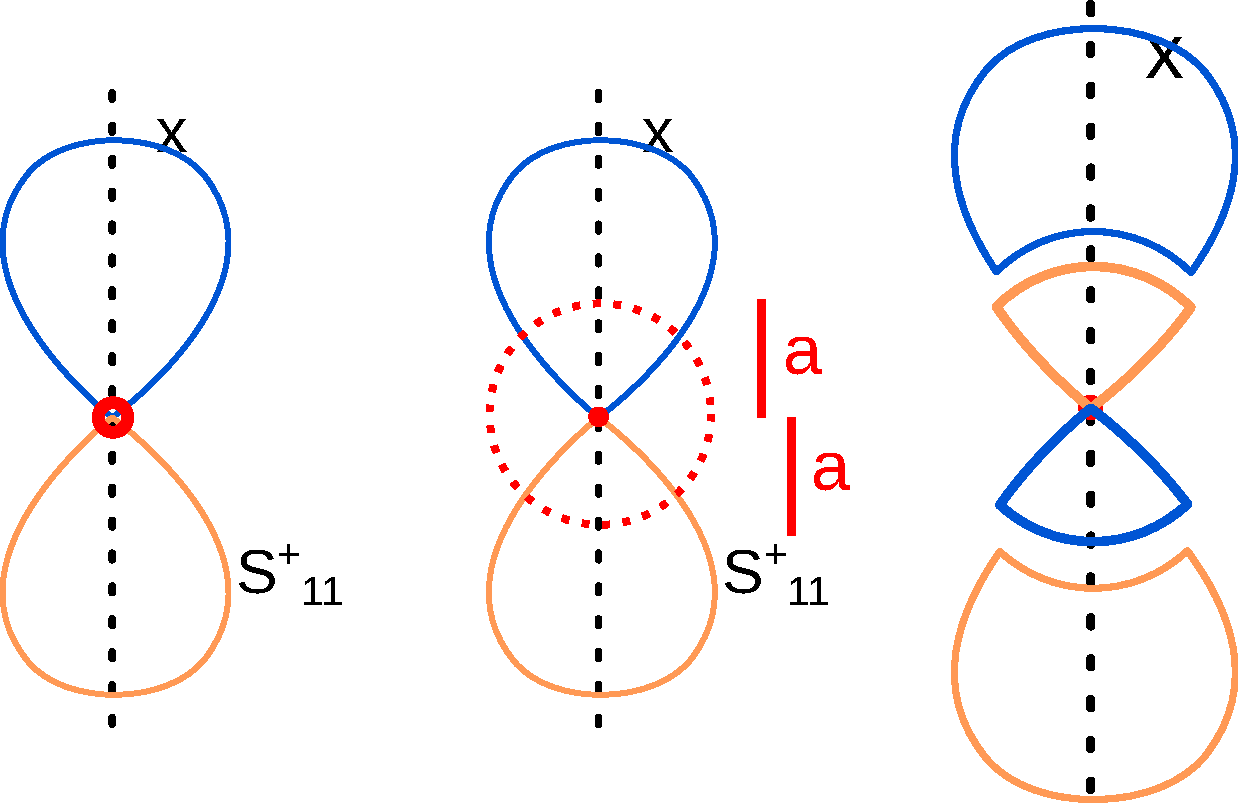
\includegraphics[scale=0.3]{2p-3p}
\section{Méthode}

\subsection{Trouver quelle formule utiliser sur la partie radiale}
 $\int_0^{+\infty} |R_{n,l}(n)|^2 r^2 dr = 1$ est utilisée pour la condition de normalisation.

 Trouver la distance électron-noyau pour laquelle la probabilité de présence est maximale. On dérive $R_{n,l}(r)^2r^2$.


\subsection{Trouver la distance électron-noyau pour laquelle la densité de probabilité de présence radiale est maximale}
\begin{enumerate}
 \item On prend la formule $R_{n,l}(r)$ de l'OA étudiée
 \item On la met au carré et on multiplie par $r^2$ : $R_{n,l}(n)^2 r^2$
 \item On dérive la fonction
 \item On factorise avec des racines évidentes ou d'autres méthodes pour trouver toutes les valeurs de $r$ où la dérivée s'annule
 \item Le maximum de probabilité est atteint pour le $r$ le plus éloigné du noyau. On classe donc les racines trouvée par taille et on prend la plus grande
\end{enumerate}

\subsection{Représenter une fonction angulaire complexe en fonction angulaire réelle}
On utilise des formules de linéarisation puis celles d'Euler\marginInfo{\[\cos(\theta) = \frac{e^{i\theta} + e^{-i\theta}}{2}\]  \[\sin(\theta) = \frac{e^{i\theta} - e^{-i\theta}}{2i}\]}

\begin{theorem}[Formule de linéarisation de la partie angulaire]
\begin{itemize}
 \item $\displaystyle S^+_{l|m|} = \frac{Y_{l,m} + Y_{l,-m}}{\sqrt{2}} $
 \item $\displaystyle S^-_{l|m|} = \frac{Y_{l,m} - Y_{l,-m}}{i\sqrt{2}} $
\end{itemize}

\end{theorem}
Exemple Pour $Y_{1,\pm1}$ :
\begin{flalign*}
S^+_{l|m|} &= \frac{Y_{l,m} + Y_{l,-m}}{\sqrt{2}}\\
&= \frac{ \frac{1}{2}(\frac{3}{2\pi})^{1/2}\sin(\theta)e^{i\varphi}  +\frac{1}{2}(\frac{3}{2\pi})^{1/2}\sin(\theta)e^{-i\varphi} }{\sqrt{2}}\\
&= \frac{ \frac{1}{2}(\frac{3}{2\pi})^{1/2}\sin(\theta)(e^{i\varphi}+ e^{-i\varphi}) }{\sqrt{2}}\\
&= \frac{ \frac{1}{2}(\frac{3}{2\pi})^{1/2}\sin(\theta)(2\cos(\varphi)) }{\sqrt{2}}\\
&= \frac{(\frac{3}{2\pi})^{1/2}\sin(\theta)(\cos(\varphi)) }{\sqrt{2}}\\
&= \frac{(\frac{3}{2\pi})^{1/2}\sin(\theta)(\cos(\varphi)) }{\sqrt{2}}\\
&= (\frac{3}{4\pi})^{1/2}\sin(\theta)(\cos(\varphi))
\end{flalign*}

\subsection{Montrer que la partie radiale est normalisée}
Il faut montrer que $\int_0^{+\infty} |R_{n,l}(n)|^2 r^2 dr = 1$

Exemple avec R de 1 et 0 :

\begin{flalign*}
\int_0^{+\infty} |R_{n,l}(n)|^2 r^2 dr &=\\
&=(\frac{Z}{a_0})^3\times 4\int_0^{+\infty} e^{-\frac{-2Zr}{a_0}} r^2 dr\\
&= (\frac{Z}{a_0})^3\times 4 \times \frac{2!}{(\frac{Z}{a_0})^3}\\
&= \frac{4\times 2}{8} = 1
\end{flalign*}

\subsection{Montrer que la partie angulaire est normalisée}
Il faut montrer que $\int_0^{\pi}\int_0^{2\pi} |Y_{l,m_l}(\theta,\varphi)|^2 \sin(\theta)d\theta d\varphi = 1$

Exemple avec Y de 0 et 0 :

\begin{flalign*}
\int_0^{\pi}\int_0^{2\pi} |Y_{l,m_l}(\theta,\varphi)|^2 \sin(\theta)d\theta d\varphi &=\\
&=(\frac{3}{4\pi}) \int_0^{\pi}\cos(\theta)^2 \sin(\theta)d\theta\int_0^{2\pi}d\varphi \\
&= (\frac{3}{4\pi}) [-\frac{1}{3} \cos ^3(x)]_0^{\pi}\int_0^{2\pi}d\varphi\\
&= (\frac{3}{4\pi}) \times 2\pi\times \frac{2}{3} = 1
\end{flalign*}

\subsection{Représenter des OA}
On utilise la fonction $S$ générée dans le cas où la fonction originale est complexe.

\subsubsection{Pour l=0}
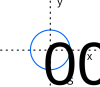
\includegraphics[scale=0.5]{s00}
\subsubsection{Pour l=1}
On dit qu'elles ont une symétrie de révolution autour d'un certain axe
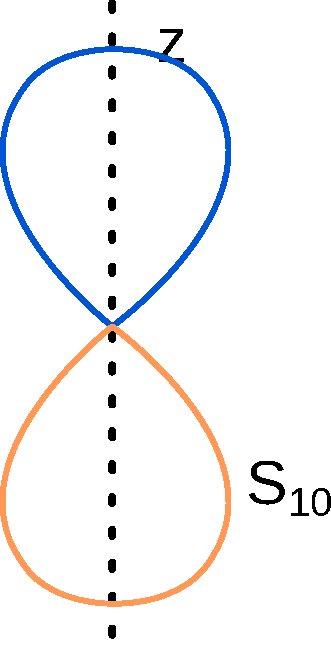
\includegraphics[scale=0.5]{s10}
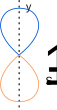
\includegraphics[scale=0.5]{s-11}
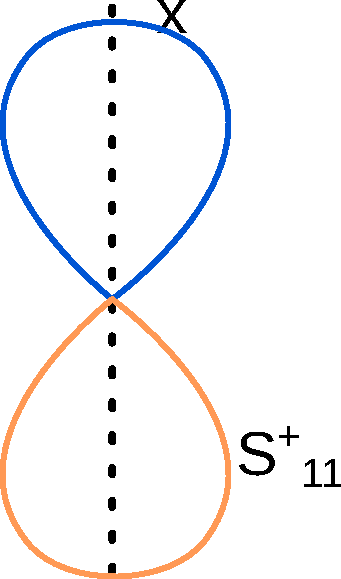
\includegraphics[scale=0.5]{s+11}
\subsubsection{Pour l=2}
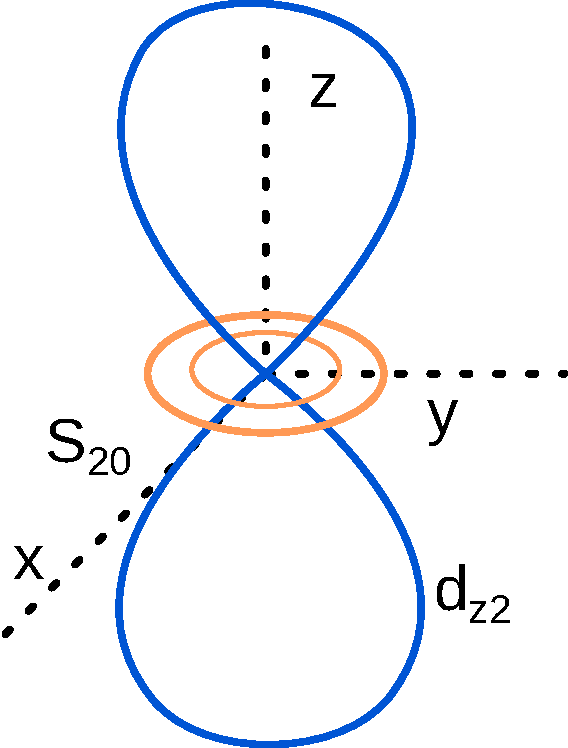
\includegraphics[scale=0.5]{s20}
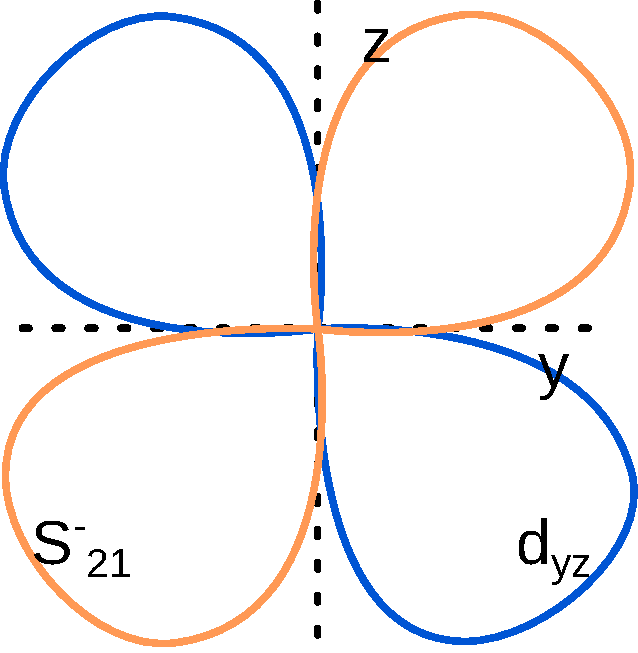
\includegraphics[scale=0.5]{s-21}
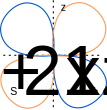
\includegraphics[scale=0.5]{s+21}
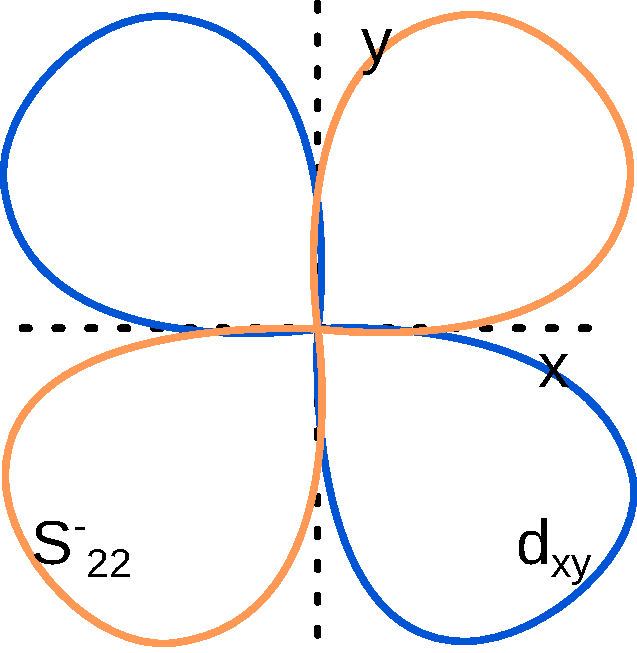
\includegraphics[scale=0.5]{s-22}
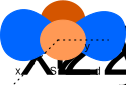
\includegraphics[scale=0.5]{s+22}


\subsection{Montrer la dégénerencexe de l'hydrogène}
\warningInfo{Dégénrences}{2 OA sont dites degénérées si elles sont la m\^eme énergie.}
\end{document}

